\section{The Fragility Issue}
\label{sec:bo}

In this section, we explain why \bo can be fragile
in CAT.


\begin{figure}[!htbp]
\centering
\begin{subfigure}[b]{0.45\textwidth}
    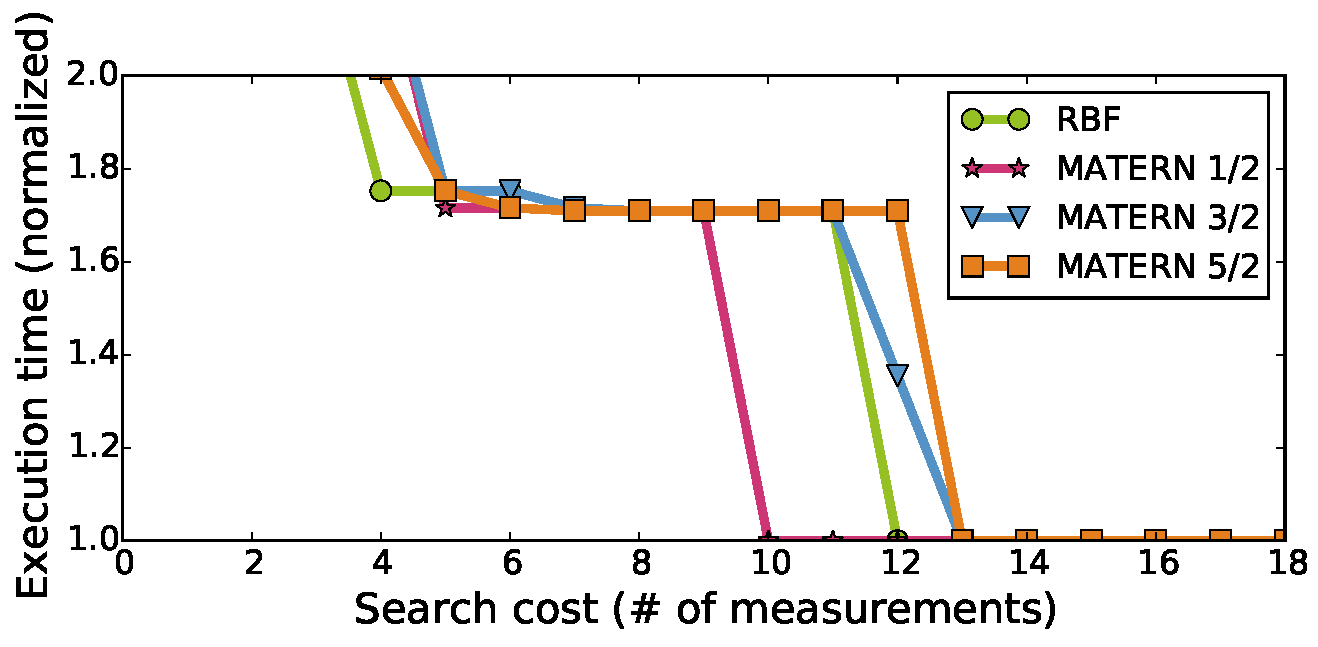
\includegraphics[width=\linewidth]{figures/kernel_time_spark.als.large_new.pdf}
    \caption{Minimizing execution time for \emph{als}}
    \label{fig:cases_good}
\end{subfigure}
\hfill
\begin{subfigure}[b]{0.45\textwidth}
    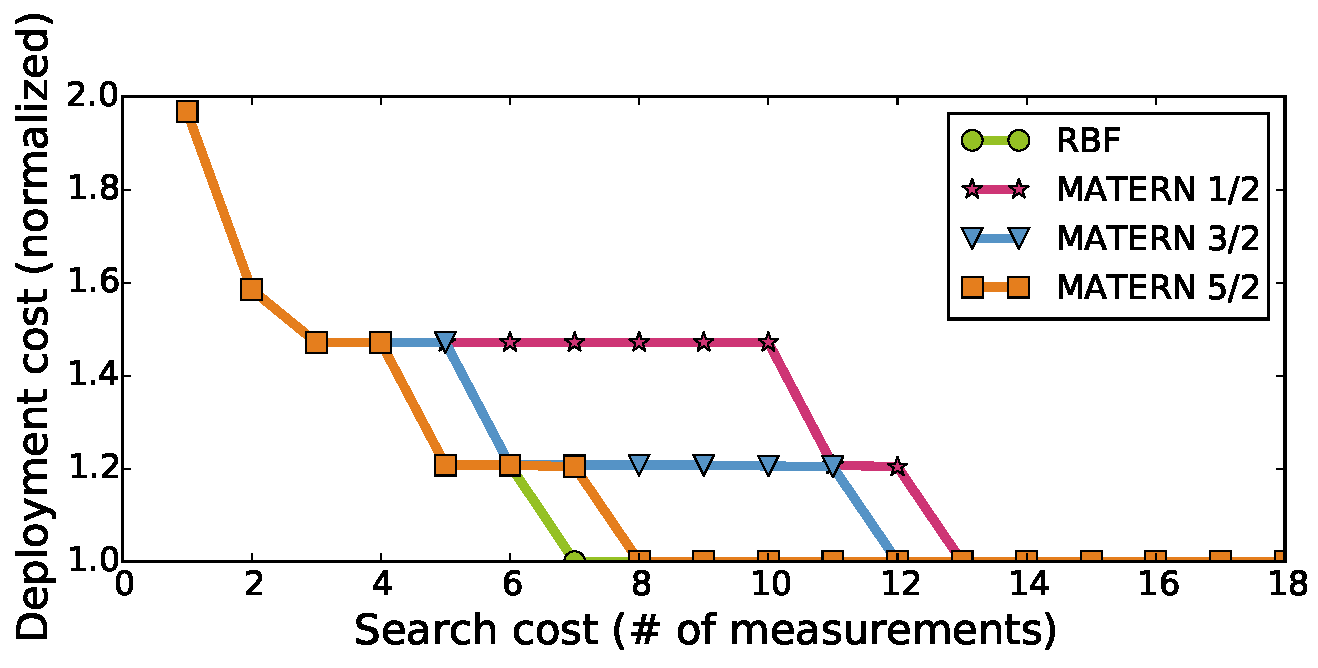
\includegraphics[width=\linewidth]{figures/kernel_cost_spark.bayes.medium_new.pdf}
    \caption{Minimizing deployment cost for \emph{bayes}}
    \label{fig:cases_bad}
\end{subfigure}
\caption{The number of actual measurements required to find
 the optimal VM type by Bayesian Optimization
 with different kernel functions.  Each kernel function is tested
 with 100 different sets of initial points uniformly selected. The points represent the median performance from 100 runs.}
\label{fig:kernel_comparison}
\end{figure}


\subsection*{Choosing the Right Kernel Function is Prone to Error}
\label{sec:kernel}
Since the choosing the covariance kernel function is critical, this section examines how different kernel functions can affect the usefulness of BO.
We implement BO (as prescribed by \emph{CherryPick}) to examine four different kernel functions.
First, \emph{RBF} (Radial Basis Function) is a widely used kernel. It considers the effects of features on the covariance equally~\cite{Brochu2010}, which may not be realistic.
\noindent {Mat\'ern} kernel function is another family of covariance functions which incorporates a smoothness parameter such that it is flexible to model different objective functions.
The smoothness parameter serves as the similarity function that determines whether two samples are alike. 
% In our setting,  it suggests that the performance difference between two VMs is less dramatic if a higher smooth parameter is used. 
The most commonly used smoothness parameters are \emph{Mat\'ern 1/2}, \emph{Mat\'ern 3/2}, and \emph{Mat\'ern 5/2}.



\myfigure{\ref{fig:kernel_comparison}} shows the number of actual measurements required to find the best VM for a given workload.
Figure~\ref{fig:cases_good} shows that
BO with \emph{Mat\'ern 1/2} kernel finds the optimal VM faster thereby reducing the search cost.
However, in Figure~\ref{fig:cases_bad}, while trying to find a cost-effective VM,
BO with \emph{Mat\'ern 1/2} kernel performs the worst.
With the two particular examples,
we want to demonstrate that choosing the appropriate kernel function affects the performance of BO.
In practice, choosing the right kernel function relies on engineering and automatic model selection~\cite{Brochu2010, Snoek2012, Dewancker2015, shahriari2016taking}.

Our prior experience indicates that it is possible to have a non-smooth performance outcome for a given workload on different VMs~\cite{Hsu2016}.
When a workload hits a resource bottleneck, \eg{memory or disk}, it can slow down greatly. This means that a workload might perform very differently on two VMs which are close to each other in the instance space. Therefore, we believe that architecture parameters alone are insufficient to predict the performance of cloud applications~\cite{Yadwadkar2017, Hsu2016}.

\subsection*{No one-size-fits-all initial points}
\label{sec:init_points}

The choice of initial VMs also affects the effectiveness of BO. A common approach is a quasi-random method which uniformly selects very distinct VMs~\cite{Sobol1998}.
This method helps capture workload behavior, which can then be used to choose the next best VM to measure.
However, in practice, we have seen that BO is sensitive to initial points (VMs in our setting) and can exhibit large variances in their outcome.

To demonstrate the effect of initial VMs on the performance of BO, we choose three very different starting points, \ie{\emph{c4.xlarge}, \emph{m4.large} and \emph{r3.2xlarge}}, and then
run BO on all the 107 workloads. We observe that about 15\% applications do not find
the optimal configuration within six attempts (33\% of the instance space). 
We choose multiple combinations of initial VMs and repeat the same experiment,
and we observe a similar phenomenon. 
This experiment shows that the performance of BO is dependent on the choice of initial VMs.
%We then redo the same experiment but choose different initial VMs. We find that
%the BO can find the optimal configuration within six attempts.
%This result demonstrates that the initial points dramatically affects the performance of BO.
% There does not exist one-size-fits-all initial points for different workloads.

Even though there exists a set of initial points that work well
on almost all applications,
the optimal initial VMs are subject to change because new VMs
are frequently added to the Cloud portfolios. Therefore, it is essential to design a search method that performs consistently with different initial points.


\subsection*{Summary}

BO is a promising technique for finding the best VM for any workload.
However, our large-scale evaluation shows that a BO method can be \textit{fragile} or unstable.
Without proper design, it may lead to high search cost or a sub-optimal solution. This is because the effectiveness of BO is significantly affected by choice of the kernel function and the initial VMs (used to seed the BO). However, choosing the suitable kernel function requires
further analysis and in-depth study.
To sum up, BO can be fragile and requires extra care while making design choices.
Our objective is to make BO less fragile by (i) augmenting BO with additional (low-level) information and (ii) use variants of BO, which are less sensitive.
